\chapter[Tensor Processing Unit]{Tensor Processing Unit}
\label{ch:tensor-processing-unit}\index{Tensor Processing Unit|(}
A Tensor Processing Unit or TPU, is a proprietary Application-Specific Integrated Circuit\index{Application-Specific Integrated Circuit } (ASIC) used as an Artificial Intelligence accelerator \citep{jouppi2017datacenter}. It is designed and built by Google for use in their datacentre to power their products, including; Google Search, Google Translate, Google Photos and Gmail. Through Google's proprietary Accelerated Linear Algebra (XLA) compiler, binaries to run on TPUs are compiled from an XLA graph format produced by the TensorFlow libraries \citep{google}. 

Note that for the scope of this documentation, the architecture of the first generation TPUs is going to be explained, since it's the most well documented one. Further updates in the architecture are fairly similar to what will be discussed here and follow the same concepts, with the main difference being that newer generations are also used for training, instead of just inference. Therefore they support a truncated variant of the IEEE 754 single-precision floating-point format called bfloat16 instead signed 8-bit integers together with various other training optimizations.

\section{Background}\label{sec:background}

The motivation for Google to design and build a custom architecture on an ASIC, is due the shortcomings that come with Central Processing Units (CPUs) and Graphics Processing Units (GPUs) when used to run Artificial Neural Network\index{Artificial Neural Network} models. This is because 95\% of Google's applications in their datacentre run Neural Networks for inference, specifically; Convolutional Neural Networks (CNNs)\index{Convolutional Neural Network}, Multi-layer Perceptron Neural Networks (MLPs)\index{Multi-layer Perceptron} and Long short-term memory Neural Networks (LSTMs)\index{lstm} \citep{jouppi2017datacenter}. 

CPUs are sequential by nature, where each instruction is executed one at a time, which is really undesirable, and would require high clock speeds to get very high performance but with the expense of higher power consumption. In contrast GPUs are concurrent by nature, meaning that they can do several concurrent operations at once, therefore eliminating the need to have very high clock speeds, but it is only well suited for vector processing, hence their main use is Graphics Processing. In Machine Learning and specifically in Neural Networks, matrix operations are preferred as they speed up the computation by quite a big margin\citep{sato}.

Additionally, modern CPU and GPU architectures have performance issues due to their complex and sometimes non-deterministic ways of executing programs. This includes complex optimizations, like branch-prediction, out-of-order execution and multiprocessing \citep{paun2013determinism}. These algorithms are more tailored for throughput efficiency rather than having fixed latency \citep{jouppi2017datacenter}. Additionally, complex algorithms implemented in modern CPUs and GPUs, together with their high clock speeds, contribute to both a large area and higher power consumption. Google therefore designed their own custom AI accelerator chip around the necessary building blocks to run their Neural Network applications on, with the maximum possible efficiency.  

In order to understand why Google TPUs are designed as they are, an insight into the mathematics of involved in Neural Networks\index{Neural Network} is needed. The only computations done in Neural Networks involve only multiplications and additions, when excluding the activation function. While CNNs\index{Convolutional Neural Network} use convolution instead of multiplication, this report will explain the multiplication operations. This is because the input of a neuron is the sum of weighted (synapse weight) outputs of all the neurons in the previous layer, as represented in Equation~\ref{neuronsumofproducts}.

\begin{equation}\label{neuronsumofproducts}
Z = \sum_{i=1}^{n}x_{i}w_{i}
\end{equation}

Where $i$ is the number of neurons in the previous layer connected to the current neuron, $x$ is the output of each individual neuron in the previous layer, $w$ is the synapse weight present in the connection between the previous neurons to the current one. 

\section{Architecture}\label{sec:architecture}

Therefore as described in the previous section, a Multiply-Accumulate\index{Multiply-Accumulate} (MAC) block is the only computational block that is needed to perform the needed operations. Figure~\ref{fig:mac} illustrates a typical MAC block, where binary values A and B of length $[n:0]$ are multiplied, therefore producing a binary value C of length $[2n+1:0]$. C is then added to the accumulated binary value Y, and the Accumulator register is updated with the new accumulated binary value. The Accumulator Register's value is present on binary value Y.

\begin{marginfigure}
  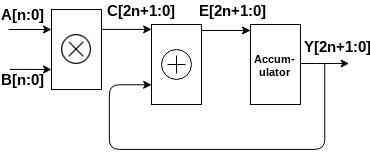
\includegraphics{graphics/tensor_processing_unit/tensor_processing_unit_mac.jpg}
  \caption{
    Multiply Accumulate Logic Block (Adapted from \citep{paquin}).
  }
  \label{fig:mac}
\end{marginfigure}

The MAC block alone does not contribute to good performance when a large data-set and complex Neural Networks are present, therefore TPUs implement it in a so called Matrix Multiplication Unit\index{Matrix Multiplication Unit} (MXU), which is basically a 2-dimensional array of MACs that operate in systolic form \citep{paquin}. The best intuitive way to understand how an MXU works is to visualize matrix multiplication as done in a layer of a Neural Network prior to activation\index{Activation Function}.

Consider the simple example shown in Figure~\ref{fig:neuralnetworkexample}, which shows a Neural Network\index{Neural Network} layer with 3 inputs and 2 neurons. Prior to applying the activation\index{Activation Function} function $f(x)$, the computation done is the same as described in Equation~\ref{neuronsumofproducts}, for each neuron, y1 and y2. 

\begin{marginfigure}
  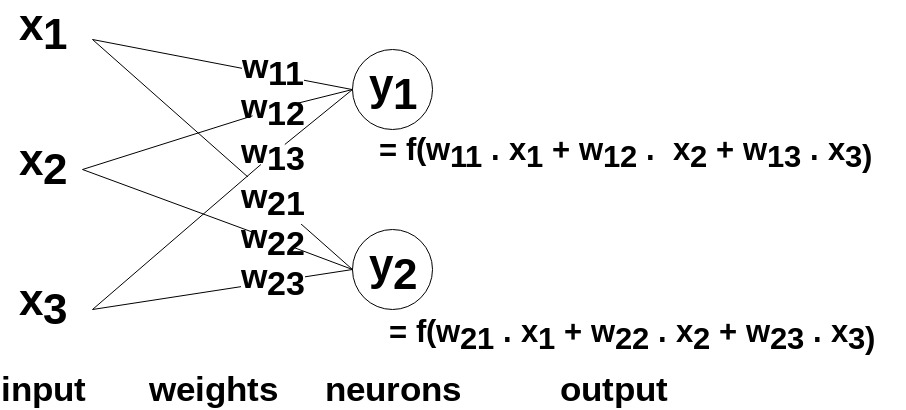
\includegraphics{graphics/tensor_processing_unit/tensor_processing_unit_nn.jpg}
  \caption{
    Example of a neural network layer with 2 neurons and 3 inputs (Reproduced from \citep{sato}).
  }
  \label{fig:neuralnetworkexample}
\end{marginfigure}

For this example an MXU needs to contain at least 6 MACs arranged in array of 2$\times$3, where 2 denotes the number of neurons and 3 denoting the number of inputs. Figure~\ref{fig:mxu} shows how such computation is done inside the MXU\index{Matrix Multiplication Unit} with just 1 example/instance X being inputted for inference, and since we are computing just 1 layer, the weights $w$ only need to be loaded once. 

\begin{figure}
  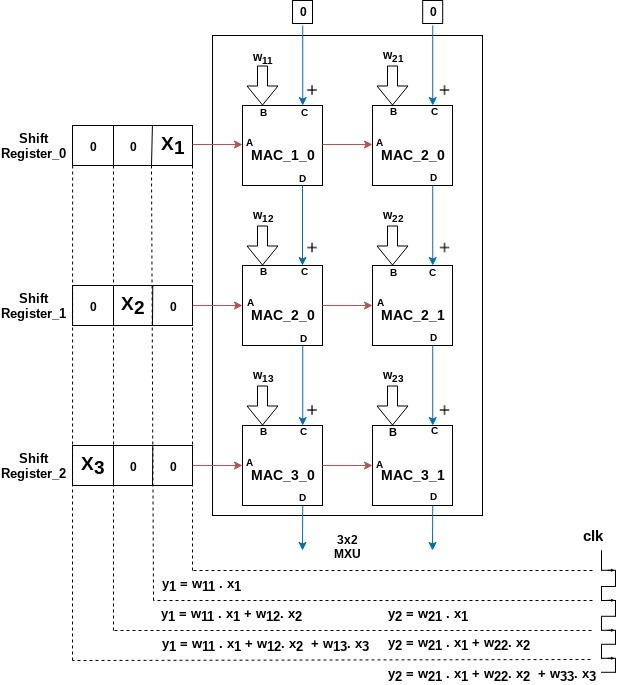
\includegraphics{graphics/tensor_processing_unit/tensor_processing_unit_mxu.jpg}
  \caption{
    Operation of a Simplified Matrix Multiplication block based on a 2 neuron layer example having 3 inputs (Adapted from \citep{sato}). 
  }
  \label{fig:mxu}
\end{figure}

Assuming input data X1, X2 and X3 are already loaded into their corresponding shift register and the weights $w$ are already present on one of their corresponding MAC inputs, the data flow with each clock cycle denoted by clk in Figure~\ref{fig:mxu}, which follows a systolic fashion. 

Prior to the computation, inputs A of all the MACs\index{Multiply-Accumulate} are reset to 0, while inputs B will have already been loaded with the weight values of the current layer. With each clock cycle the shift registers shift the data to the right into the MXU, where the A and B inputs are multiplied together and added with the value present at input C. In this manner the values of outputs D of the bottom most MACs will output the total sum of products on output D, with the bottom right most MAC being the last one to be updated after \textit{mn-m} clock cycles, where m is the number of inputs and n is the number of neurons. In this example the total amount of clock cycles needed is $2$ $\times$ $3$ $-$ $2$ $=$ $4$. In a Google's first generation TPU, there are 65,536 signed 8-bit MAC blocks in a 256$\times$256 array fashion that make up the MXU. The MXU in a TPU can compute both matrix multiplication and convolution \citep{sato}. After finally computing the sum of products, activation functions\index{Activation Function} are applied on each neuron's result.

Figure~\ref{fig:layouttpu} shows a high level representation of how all the components of the first generation TPU are connected internally, including the MXU\index{Matrix Multiplication Unit}. TPUs where designed to act as coprocessor with a host CPU, where they communicate together via a 3rd generation PCIe x16 bus. First generation TPUs were only designed for inference only, therefore the TPUs represent data only in a signed 8-bit integer, which has been proved that it is of sufficient precision for inference purposes \citep{jouppi2017datacenter}. 

\begin{figure}
  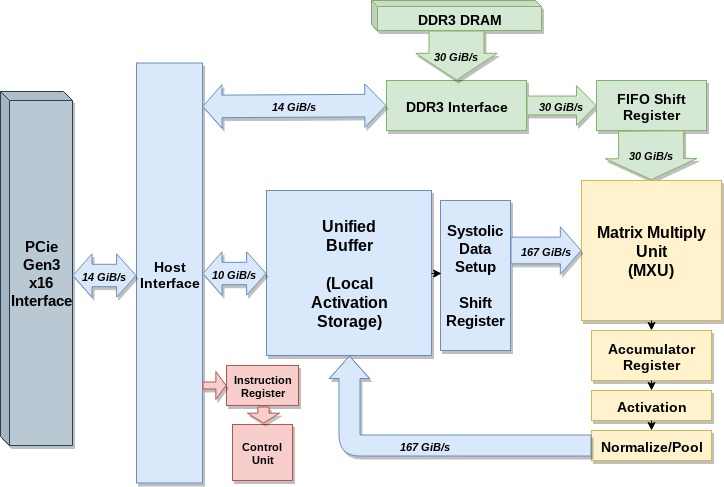
\includegraphics{graphics/tensor_processing_unit/tensor_processing_unit_arch.jpg}
  \caption{
    Internal Layout of a first generation TPU, showing the Control path (red), the Data paths for the weights (green) and for the activations/outputs (blue), together with the computational logic blocks (yellow) (Adapted from \citep{sato}).
  }
  \label{fig:layouttpu}
\end{figure}

As with any architecture, there is a Control path and a Data path. The Control path, which is denoted in red, serves the purpose of giving instructions to the TPU via the host CPU, like loading the data in registers, do multiplication and more. As for the Data path, two types of data are present. One being the weights, which are stored prior of inference and are denoted in green, while the other is the neurons activations/outputs, where its path is denoted in blue. As the weights are loaded only once before computing each layer, they do not require a high speed memory, so they are stored in a DDR3 DRAM, where later they are loaded into the MXU via a FIFO shift register. On the other hand, the neuron's activations/outputs, are stored by the host CPU in a high speed Unified Buffer through the PCI Express Interface. The Unified Buffer is where the activations of each neuron that are computed by the computational logic block are read and written, therefore it requires a high speed memory and interconnect bus. The Normalize/Pool block, processes the data to reduce its size or downsample it. As one can see the architecture is quite simple compared to other general purpose architectures like CPUs and GPUs. This allows Google to use a Complex Instruction Set Computer (CISC) instruction set with just a few instructions, since not many different operations are done \citep{sato}.

\index{Tensor Processing Unit|)}
